\chapter{Metodologia}
	\chapterprecis{Este capítulo apresenta a arquitetura do sistema implementado. Primeiramente, são descritos os requisitos funcionais do sistema, que orientam a montagem da estrutura. São definidos os componentes do sistema e suas interconexões, sendo que esta definição é acompanhada de um breve descritivo do funcionamento.}
	
	\section{Estado Atual}
	
		A Arquitetura do sistema atual instalado na planta de trocador de calor está representada na \autoref{img3}. Pelo painel é possível efetuar a leitura das variáveis de processo, cuja leitura é feita pelo Arduino, bem como comandar a bomba e o aquecedor. É importante observar que o controle da potência do aquecedor não passa pelo Arduino, e que o sistema não recebe nenhum feedback sobre a velocidade da bomba, bem como sobre a potência do aquecedor. Apesar de estar previsto no projeto de \textcite{luiz2016}, nenhum controle em malha fechada está operacional.
		
		
	
		O intuito do projeto é implementar um sistema de monitoramento e controle remoto, sem que haja alteração infraestrutura já montada. Em resumo, o objetivo é implementar um sistema que necessite apenas se comunicar com o Arduino para executar as suas tarefas.
	
	
	\section{Requisitos Funcionais do Sistema}
		Para determinar a arquitetura do sistema a ser implementado, foram levantados os requisitos funcionais do sistema, ou seja, quais informações devem ser transmitidas ao operador, bem como quais as ações que este pode realizar no sistema. Os requisitos estão resumidos na \autoref{tbl1}.
		
		% Please add the following required packages to your document preamble:
		% \usepackage{booktabs}
		\begin{table}[!htb]
			\centering
			\caption{Requisitos Funcionais do Sistema}
			\label{tbl1}
			\def\arraystretch{1.3}
			\begin{tabular}{c p{11cm}}
				\hline
				\multicolumn{1}{c}{\textbf{Índice Requisito}} & \multicolumn{1}{c}{\textbf{Descrição Requisito}} \\ \hline 
				1 & Exibir a informação atual das variáveis de processo (vazões e temperaturas) \\ %\hline
				2 & Exibir o estado da bomba e do aquecedor (Ligado ou Desligado) \\ %\hline  
				3 & Exibir o valor da rotação atual da bomba \\ %\hline
				4 & Em modo remoto, deve permitir que o operador acione a bomba e o aquecedor \\ %\hline
				5 & Em modo remoto, deve permitir que o operador altere a velocidade da bomba \\ %\hline
				6 & Permitir a visualização dos dados analógicos em gráficos \\ %\hline
				7 & Impedir a atuação do operador quando o Arduino estiver em modo local ou de emergência \\ %\hline
				8 & Armazenar os dados do sistema em banco de dados \\ %\hline
				9 & Permitir que o usuário habilite ou desabilite o armazenamento de dados das variáveis \\ %\hline
				10 & Permitir que o usuário colete as informações contidas no banco em um arquivo no formato csv \\ %\hline
				11 & Permitir que o usuário apague as informações contidas no banco de dados \\ \hline
			\end{tabular}
		\end{table}
	
		Após levantamento dos requisitos, é possível concluir que as arquiteturas citadas na \autoref{sec:rev_monitor} podem ser utilizadas. É possível utilizar um PC que executa um software SCADA tradicional como utilizado por \textcite{alexandre2015}. Basicamente, o Arduino foi programado de forma que ele consiga utilizar um protocolo industrial comumente utilizado por ferramentas SCADA, no caso o protocolo Modbus\footnote{\url{http://www.ni.com/white-paper/52134/pt/}} foi utilizado. Também é possível utilizar uma arquitetura totalmente embarcada como utilizada no sistema \textit{BrewPi} \cite{brewpi}.
	
	\section{Critérios para Escolha do Sistema}
		Para possibilitar a comparação entre a arquitetura SCADA tradicional e embarcada e consequentemente ajudar na tomada de decisão, algumas características pontuais do sistema foram avaliadas. Existem características subjetivas e objetivas, sendo que as características subjetivas foram avaliadas de acordo com a experiência na utilização das ferramentas pelo desenvolvedor. Como existem diversos softwares SCADA no mercado, um software específico foi escolhido para comparação. O E3, que é fornecido pela Elipse Software\footnote{\url{https://www.elipse.com.br/produto/elipse-e3/}}, foi escolhido devido ao grau de conhecimento do desenvolvedor sobre a ferramenta. Os critérios e avaliações estão apresentados na \autoref{tbl2}.
		
		\begin{table}[!htb]
			\centering
			\caption{Comparação entre tecnologias}
			\label{tbl2}
			\def\arraystretch{1.5}
			\begin{tabularx}{\textwidth}{p{7cm} | c c}
				\hline
				\diagbox{\textbf{Critério}}{\textbf{Arquitetura}} & \multicolumn{1}{c}{\textbf{SCADA (E3)}} & \multicolumn{1}{p{5cm}}{\textbf{Tecnologia Embarcada}} \\ \hline
				
				\textcolor{blue}{Custo} & \multicolumn{1}{c}{Alto} & \multicolumn{1}{c}{Baixo} \\
				
				\textcolor{blue}{Complexidade do desenvolvimento das interfaces gráficas} & \multicolumn{1}{c}{Baixa} & \multicolumn{1}{c}{Alta} \\
				
				\textcolor{blue}{Complexidade da implementação da comunicação com Arduino} & \multicolumn{1}{c}{Baixa} & \multicolumn{1}{c}{Média} \\
				
				\textcolor{blue}{Facilidade para interoperar com outros sistemas} & \multicolumn{1}{c}{Média} & \multicolumn{1}{c}{Alta} \\ 
				
				\textcolor{blue}{Multiplataforma} & \multicolumn{1}{c}{Não} & \multicolumn{1}{c}{Sim} \\
				
				\textcolor{blue}{Interface se adapta à resolução do dispositivo} & \multicolumn{1}{c}{Não} & \multicolumn{1}{c}{Sim} \\
				
				\textcolor{blue}{Suporte a vários clientes conectados simultaneamente} & \multicolumn{1}{c}{Sim} & \multicolumn{1}{c}{Sim} \\
				
				\textcolor{blue}{Consumo de energia} & \multicolumn{1}{c}{Médio} & \multicolumn{1}{c}{Baixo} \\
						
				\hline
			\end{tabularx}
		\end{table}
	
		A grande disparidade entre esses sistemas basicamente é o custo em a relação a demanda de mão-de-obra especializada para desenvolvimento de sistemas embarcados. Conhecimentos de ferramentas SCADAs já estão difundidos, facilitando o desenvolvimento de aplicações utilizando essas ferramentas. Contudo, esses softwares são caros, com exceção de algumas ferramentas \textit{opensource} como por exemplo o SCADABR\footnote{\url{http://www.scadabr.com.br/}}.
		
		Desde o início da modernização do laboratório, o custo era uma das restrições mais fortes, o que favoreceu a opção pela tecnologia embarcada. Além disso, a oportunidade de utilizar tecnologias emergentes no monitoramento de processos contribuiu ainda mais para a utilização de sistemas embarcados.
		
	\section{Arquitetura do Sistema}
		A arquitetura pensada para o sistema foi inspirada no projeto BrewPi. Esse sistema foi concebido para controlar a temperatura de um recipiente com líquido, bem como para permitir o monitoramento via qualquer dispositivo que possua um navegador Web. A Arquitetura deste sistema é mostrada na \autoref{fig:arq_brewpi}. Basicamente, o Arduino, é encarregado de executar a malha de controle e enviar as informações para um RaspberryPi, que implementa um WebServer. Os usuários que desejam visualizar e/ou modificar as informações, devem abrir um navegador e se conectar ao WebServer para obter os dados.
		
		\begin{figure}[!htb]	
			%\centering
			\captionsetup{justification=centering}
			\begin{center}
				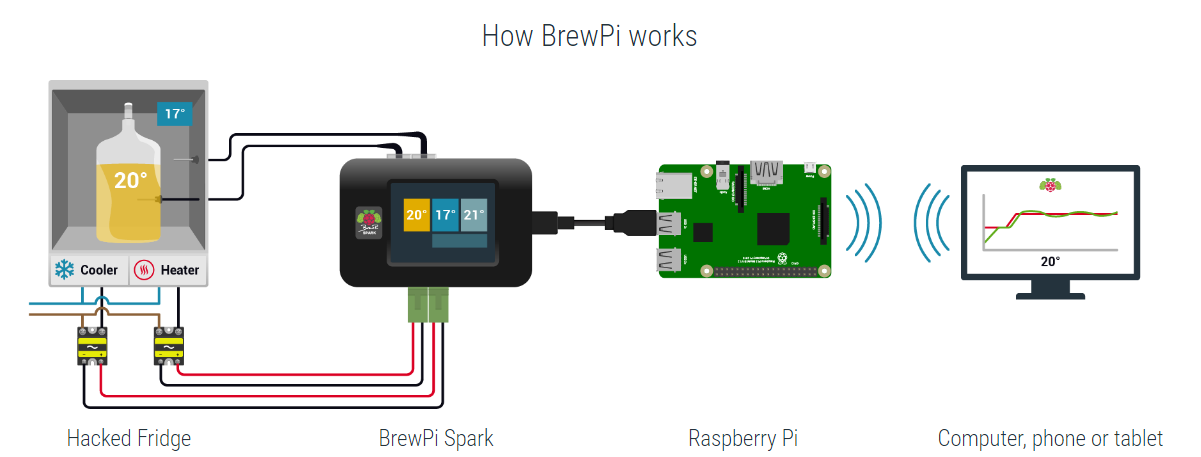
\includegraphics[width=14cm]{arq_brewpi}  %pode alterar o tamanho
				\caption[Arquitetura do sistema BrewPi]{\label{fig:arq_brewpi}Arquitetura do sistema BrewPi. Fonte: \url{https://www.brewpi.com/} }
			\end{center}		
		\end{figure}
	
		Para o trocador de calor, a proposta é semelhante. A adição de um RaspberryPi no sistema atual é simples de ser realizada e está em conformidade com a condição de não modificar as instalações atuais. Dessa forma, a arquitetura proposta simplificada para o sistema com o Raspberry é exibida na \autoref{fig:arq_proposta}. A Arquitetura detalhada do sistema, como por exemplo, os softwares a serem desenvolvidos em cada dispositivo, bem como a forma de interação entre eles serão tópicos abordados posteriormente.
		
		\begin{figure}[!htb]	
			%\centering
			\captionsetup{justification=centering}
			\begin{center}
				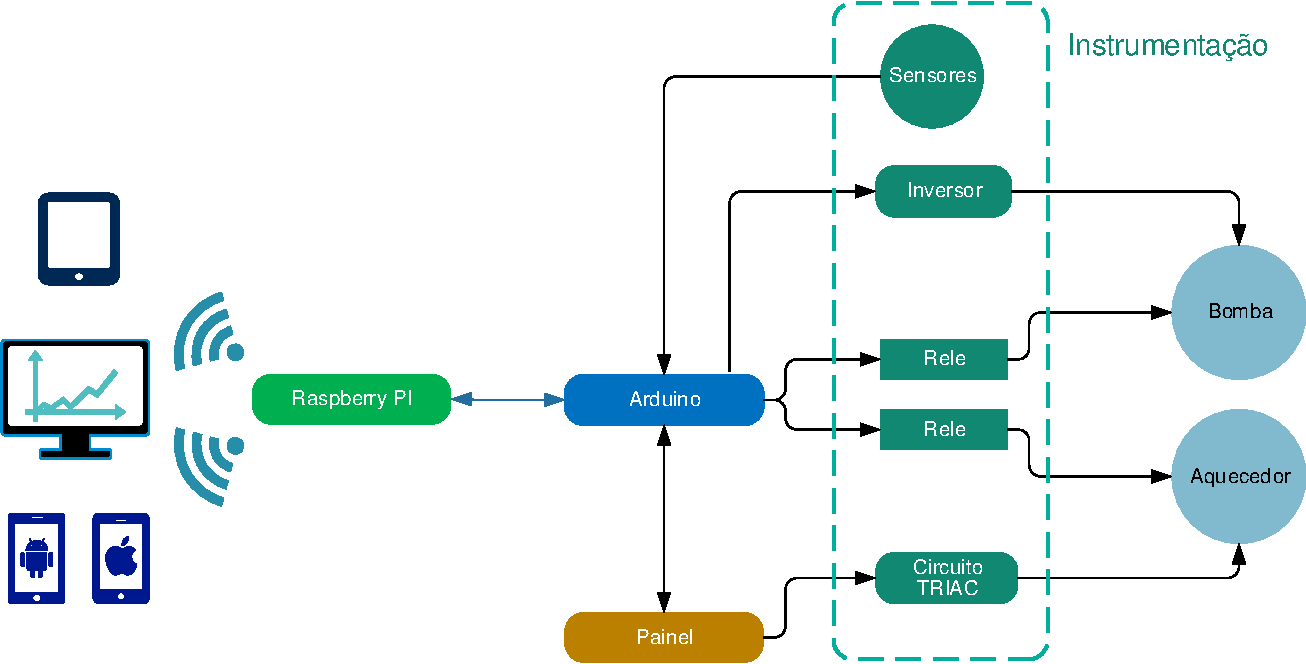
\includegraphics[width=14cm]{arq_proposta}  %pode alterar o tamanho
				\caption[Nova Arquitetura Proposta para o Sistema]{\label{fig:arq_proposta} Nova Arquitetura Proposta para o Sistema }
			\end{center}		
		\end{figure}
		
		É importante salientar que existem outros dispositivos simulares ao Raspberry PI como o BeagleBone Black\footnote{\url{https://beagleboard.org/black}} e a recente e também poderosa placa DragonBoard 410c\footnote{\url{https://developer.qualcomm.com/hardware/dragonboard-410c}}. Qualquer uma das placas poderia ser utilizada no projeto. A escolha do Raspberry PI foi influenciada pela extensa base de conhecimento e documentação já produzida pelos usuários, aliado ao menor custo da placa.  As demais placas por serem mais novas, não dispõem de muitos documentos e exemplos, o que aumenta o tempo de desenvolvimento de um novo projeto.
		
		Ainda em relação as placas utilizadas, verifica-se que existem vários modelos distintos de Raspberry PI. Portanto é necessário definir qual a versão é a mais adequada ao projeto.
		
		\subsection{Escolha da Versão do Raspberry PI}
			O Raspberry PI possui algumas versões, que se diferem em tamanho, capacidade de memória, processamento e componentes. Um resumo das características das principais versões do Raspberry é exibido na \autoref{tbl3}
			
		
		
			A última versão do Raspberry apresenta uma grande vantagem por possuir Wifi nativamente. Isso evita a utilização de adaptadores para utilizar a comunicação Wireless no dispositivo. Além disso, possui maior poder de processamento, conta com um chip mais moderno, e suporta uma capacidade maior de corrente em estado de sobrecarga. Portanto, o Raspberry 3 foi escolhido. Na próxima seção detalhados os sistemas a serem executados dentro do Raspberry e como estes se relacionam entre si e com o Arduino.
			
		\subsection{Arquitetura Detalhada do Sistema}
			A \autoref{img3} exibe a visão geral do sistema, ou seja, não exibe como é a comunicação entre os componentes. Como dito anteriormente, não faz parte do escopo do projeto promover alterações nas instalações atuais, portanto, é necessário focar apenas em como o Raspberry será programado e como será realizada a sua comunicação com o Arduino.
			
			Os componentes foram projetados de forma que cada um funcione da forma mais independente possível. Dessa forma, o impacto no sistema caso haja alguma alteração de componente, em termos de esforço de desenvolvimento, é minimizado.
			
			A arquitetura detalhada do sistema é exibida na \autoref{fig:arq_componentes}. Foram definidos 3 componentes: o programa que é executado no Arduino; o Gateway e o WebServer, \textcolor{red}{que são} programas que são executados no Raspberry. O termo componente deve ser entendido nesse contexto como um programa, por isso o banco de dados não deve ser interpretado como um componente. Optou-se por criar dois programas no Raspberry PI, de forma que as funcionalidades do sistema fossem corretamente agrupadas. As atribuições de cada programa estão resumidas na \autoref{tbl4}
			
			\begin{table}[!htb]
				\centering
				\captionsetup{justification=centering}
				\caption[Atribuições de cada Componente]{Atribuições de cada Componente}
				\label{tbl4}
				\def\arraystretch{1.5}
				\begin{tabular}{m{2cm}| p{12cm}}
					& \multicolumn{1}{c}{\textbf{Atribuições}} \\ \hline
					
					\multirow{4}{*}{Arduino} 
					& 1 - Interface com sensores e Atudadores \\
					& 2 - Interface com Painel \\
					& 3 - Enviar estado do sistema quando solicitado pelo Gateway\\
					& 4 - Interpretar comandos enviados pelo Gateway \\ \hline
					
					\multirow{3}{*}{Gateway} & 5 - Solicitar de forma cíclica o estado das variáveis \\
					& 6 - Armazenar os dados recebidos em um banco de dados \\
					& 7 - Receber comandos vêm do WebServer (comandos dos usuários) e repassar ao Arduino \\ \hline
					
					\multirow{2}{*}{WebServer} & 8 - Ler dados do banco e apresentar ao usuário \\
					& 9 - Receber comandos do usuário e repassar ao Gateway \\
						
					\hline
				\end{tabular}
			\end{table}
			
			\begin{figure}[!htb]	
				%\centering
				\captionsetup{justification=centering}
				\begin{center}
					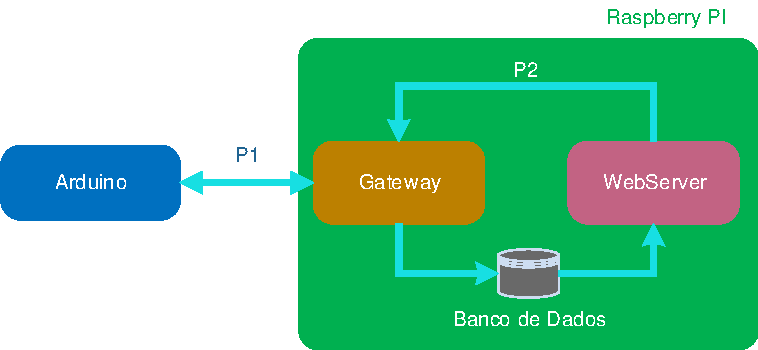
\includegraphics[width=12cm]{arq_componentes}  %pode alterar o tamanho
					\caption[Arquitetura Detalhada]{\label{fig:arq_componentes} Arquitetura Detalhada }
				\end{center}		
			\end{figure}
		
			É importante observar que as atribuições 4 e 5 envolvem uma comunicação entre Arduino e Gateway, e as atribuições 7 e 9 envolvem uma comunicação entre o WebServer e Gateway. Portanto, é necessário definir protocolos de comunicação para ambos os casos. Já foi dito que os componentes foram projetados de forma a possibilitar a substituição de um componente sem alterar os demais. Porém, alterações no protocolo de comunicação necessariamente levam a modificações nos componentes envolvidos. Em resumo, os protocolos de comunicação devem ser mantidos.
			
			
			\subsubsection{Funcionamento do Arduino}
				\label{sec:met_arduino}
				Foi feita uma análise do programa atual que o Arduino executa. O programa é extenso (contém 1482 linhas), sendo que cerca de 90\% do código é dedicado a cuidar do sistema de navegação do display LCD através dos botões existentes no painel.  A implementação de um sistema de monitoramento elimina a necessidade dessa estrutura de navegação, de modo que o painel passe a ter apenas funcionalidades diretas de acionamento, e o display exiba apenas informações básicas. Portanto, a melhor opção foi reformular o código do Arduino e aproveitar apenas as funções que fazem a leitura dos sensores e convertem os valores para unidade de engenharia.
				
				A estrutura do código, que está exibida na \autoref{fig:fluxo_arduino}, foi montada de forma a permitir rápida adaptação do mesmo para diferentes protocolos de comunicação, e está de acordo com as atribuições mencionadas na \autoref{tbl4}. As trocas de mensagens com o Gateway são feitas por interrupção, ou seja, estão fora da função \textit{loop} do Arduino. 
				
				O programa criado seguiu o paradigma de programação procedural, ou seja, o programa foi bastante modularizado. Esse tipo de prática acelera a identificação de uma funcionalidade (atribuição) no código fonte, o que facilita a manutenção deste. Outro benefício é a possibilidade de expansão de funcionalidades, como por exemplo a implementação de malhas de controle no código. \textcolor{red}{ Para isso, um Estado Automático cujas atribuições fossem executar as malhas de controle poderia ser adicionado ao sistema. Para que este estado entre em funcionamento, bastaria adicionar mais uma condição de teste no código, ou seja, uma alteração bastante simples.}
				
				No diagrama é utilizado o termo ``estado do sistema'', que deve ser interpretado como o conjunto de variáveis necessários para descrever o sistema. Essas variáveis são: as 4 temperaturas; 2 vazões; estado de acionamento de bomba e aquecedor (Ligado ou Desligado); velocidade da bomba; modo de operação (Local ou Remoto) e se o botão de emergência está acionado ou não.
			
				\begin{figure}[!htb]	
					%\centering
					\captionsetup{justification=centering}
					\begin{center}
						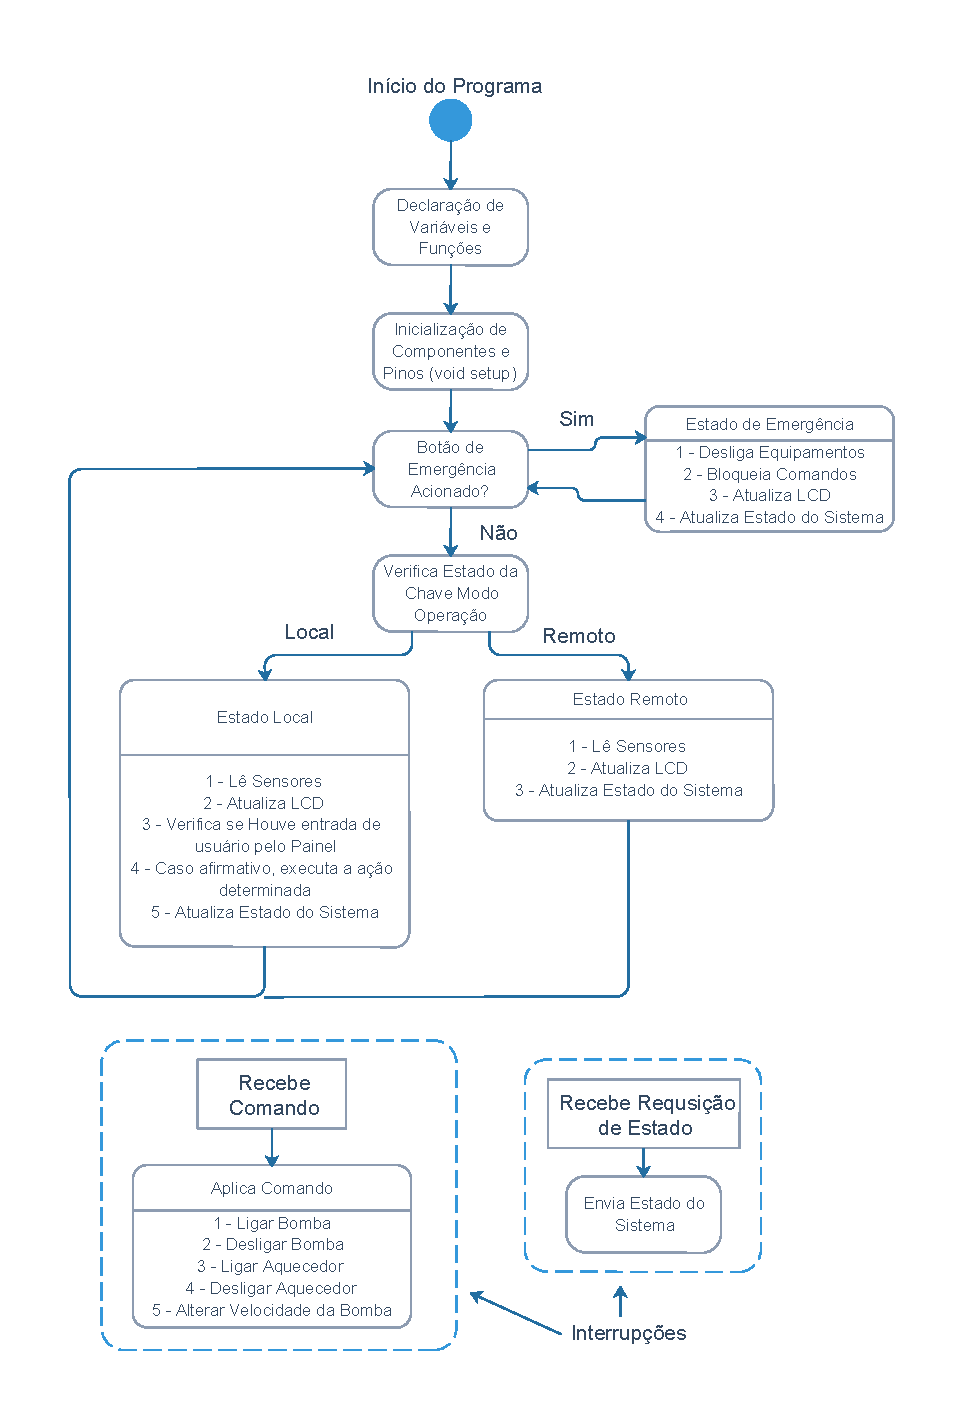
\includegraphics[width=12cm]{fluxo_arduino}  %pode alterar o tamanho
						\caption[Estrutura do Código do Arduino]{\label{fig:fluxo_arduino} Estrutura do Código do Arduino }
					\end{center}		
				\end{figure}
			
			\subsubsection{Comunicação Entre Arduino e Gateway}
				Ao observar as atribuições 3 e 4 da \autoref{tbl4}, verifica-se que a comunicação entre Arduino e Gateway é do tipo mestre-escravo, ou seja, o dispositivo mestre (Gateway) sempre inicia a comunicação, e o escravo (Arduino) responde quando solicitado. Existem diversos protocolos que implementam esse tipo de comunicação.
				
				É necessário escolher um protocolo que funcione em meio físico serial, uma vez que nenhum \textit{Shield} Ethernet será utilizado. É possível portanto utilizar algum protocolo industrial, disponibilizado na forma de bibliotecas, ou então algum dos protocolos seriais descritos na seção \textcolor{red}{colocar aqui a seção da rev sobre protocolos}, ou seja: UART, SPI, I2C.
				
				O protocolo industrial aberto encontrado com maior frequência em outras referências e implementações é o Modbus. É possível baixar pelo menos 5 bibliotecas que implementam o protocolo. A utilização de Modbus apresenta a vantagem de facilitar a integração com diferentes sistemas, uma vez que é um protocolo amplamente difundido e utilizado. Contudo, ao adicionar a biblioteca Modbus no Arduino, o código aumenta consideravelmente o tamanho, pois as bibliotecas implementam praticamente todo o protocolo, o que é desnecessário para o projeto atual, uma vez que a quantidade de informações trafegadas entre os componentes é pequena.
				
				O protocolo SPI possui uma taxa de transferência máxima maior que I2C e UART, porém a implementação da troca das mensagens entre os dispositivos é a mais complexa. O protocolo SPI exige o recebimento de informação enquanto está enviando, o que é ruim em para o propósito desse sistema, pois torna-se necessário o tratamento de informações indesejadas. A comunicação UART permite a implementação mais simples de troca de mensagens. Porém, é a mais lenta das 3, além de ser assíncrona. Além disso, a troca de mensagens é através de strings, portanto, o tamanho dos frames envolvidos na troca de mensagens é maior. 
				
				O protocolo I2C se apresenta como um meio termo entre SPI e UART, em termos de complexidade das trocas de mensagens e velocidade de comunicação. Além disso, é um protocolo síncrono, e a velocidade típica de utilização, que é 100kbps, atende plenamente ao projeto.
				Portanto, o I2C será utilizado no projeto. Existe uma biblioteca nativa que implementa o I2C para o Arduino, bem como existem bibliotecas I2C para diversas linguagens de programação (necessário para o Gateway). Os detalhes dos frames de comunicação serão explorados no capitulo de \textcolor{red}{implementação}.
			
			\subsubsection{Funcionamento do Gateway}
				\label{sec:met_gateway}
				O programa do Gateway foi desenvolvido em Python, embora possa ser escrito também em Java e C/C++, que são linguagens também suportadas pelo Raspberry. O Python foi escolhido por ser uma linguagem de programação de alto nível, ou seja, uma linguagem que está próxima da linguística humana. Essa característica facilita o entendimento de programas, e acelera o processo de aprendizado da mesma.
				
				O processo do Gateway foi dividido em duas Threads. Uma thread é responsável por solicitar os dados do arduino e enviar ao banco de dados, e a outra responsável por aguardar comandos vindos do WebServer, e repassar ao Arduino. A divisão se mostra uma decisão acertada. Enquanto a tarefa de leitura dos dados e envio ao banco é executada em um intervalo fixo, o recebimento dos dados do WebServer é essencialmente assíncrono, pois os usuários podem enviar comandos em qualquer momento. Portanto, implementar ambas as funcionalidades em uma única Thread seria inviável. Além disso, essa implementação permite o repasse do comando enviado pelo WebServer para o Arduino tão logo a mensagem seja recebida. As Threads compartilham apenas um recurso, que é o canal I2C, para escrita e leitura dos dados para o Arduino.
				
				\textcolor{red}{Vale a pena colocar uma imagem para ilustrar o que foi dito no texto?}
			
			\subsubsection{Comunicação entre WebServer e Gateway}
				A comunicação entre WebServer e Gateway é feita via TCP/IP. Uma das threads do Gateway implementa um servidor TCP assíncrono que fica ``escutando'' em uma determinada porta. A cada comando de usuário, o WebServer abre um cliente, se conecta ao servidor TCP, envia a informação necessária e posteriormente fecha a conexão. Dessa forma, evita-se manter conexões estabelecidas de forma desnecessária. A linguagem Python possui pacotes que implementam servidores e clientes TCP, ou seja, o desenvolvedor não necessita se preocupar com detalhes de implementação do protocolo. Sendo assim, o foco está apenas no conteúdo das mensagens envolvidas.
				
				As mensagens trafegadas consistem em um conjunto strings. Para simplificar o processo de decodificação da mensagem, bem como facilitar a captura de erros no transporte, decidiu-se transmitir as informações em pacotes JSON. Como dito na seção \textcolor{red}{colocar aqui a seção que fala sobre json}, uma das vantagens de se utilizar JSON é a fácil interpretação das mensagens, tanto pelos humanos, quanto pelos softwares.
				
			\subsubsection{WebServer}
				Conforme foi abordado na seção \textcolor{red}{colocar a seção sobre frameworks web}, existem frameworks web para diversas linguagens de programação, inclusive existem muitos frameworks para uma mesma linguagem de programação. A linguagem Python foi mantida para o desenvolvimento do WebServer, pelos mesmos motivos mencionados na seção anterior.
				
				\textcite{bogdan2017} e \textcite{ryan2015} abordam sobre as diferenças entre os diversos frameworks web existentes para a linguagem Python. O framework escolhido foi o Django devido a 4 motivos: 
				
				\begin{enumerate}
					\item 
					É um dos frameworks mais utilizados. Portanto, conta com uma vasta e completa documentação. 
					\item 
					A complexidade de uma aplicação escrita em Django é praticamente uniforme. Ou seja, uma aplicação de pequeno porte ou grande porte, resultam em um código de complexidade próxima.
					\item 
					O framework Django é adequado para usuários	que querem desenvolver aplicações web rapidamente, sem fazer muitas decisões sobre a infraestrutura da aplicação. Ou seja, o Django já fornece uma infraestrutura básica para possibilitar desenvolvimento imediato
					\item 
					Consultas a banco de dados não precisam ser feitas utilizando código SQL. O Django provê uma estrutura de forma que é possível manipular dados do banco através de códigos Python. Isso facilita, por exemplo, algumas funcionalidades do Gateway.
				\end{enumerate}
			
				Para apresentação da interface para o cliente são utilizadas as linguagens HTML e CSS. A parte da animação e interatividade da página é desenvolvida utilizando JavaScript. Essas 3 linguagens são utilizadas por quase todos os sistemas web existentes atualmente.
				